% MVAA 2026 challenge method paper -- ANONYMIZED for double-blind review.
% Springer LNCS (llncs) -- do not modify fonts, margins, or spacing.
%
\documentclass[runningheads]{llncs}
%
\usepackage[T1]{fontenc}
\usepackage{graphicx}
\usepackage{amsmath}
\usepackage{booktabs}
%
\begin{document}
%
\title{Semi-Supervised nnU-Net with Weak--Strong Consistency and
Boundary Refinement for Mitral Valve Segmentation}
%
\titlerunning{Semi-Supervised nnU-Net for Mitral Valve Segmentation}
\author{Durgesh Kumar Singh\inst{1}\orcidID{0000-0002-4677-6854} \and
Sarina Thomas\inst{2}\orcidID{0000-0002-1202-0856} \and
Qing Cao\inst{3} \and
Michael C. Kampffmeyer\inst{4} \and
Robert Jenssen\inst{4} \and
Anne Schistad Solberg\inst{1}\orcidID{0000-0002-6149-971X}}
%
\authorrunning{D. K. Singh et al.}
%
\institute{University of Oslo, Oslo, Norway\\
\email{\{durgeshs,anne\}@ifi.uio.no}
\and
GE Healthcare, Oslo, Norway\\
\email{sarina.thomas@gehealthcare.com}
\and
GE Healthcare, Wuxi, China\\
\email{qing.cao@gehealthcare.com}
\and
UiT The Arctic University of Norway, Troms{\o}, Norway\\
\email{\{michael.kampffmeyer,robert.jenssen\}@uit.no}}
\maketitle
%
\begin{abstract}
Automatic segmentation of the mitral valve can reduce manual work and
support faster image analysis. The MICCAI 2026 Mitral Valve Anatomy
Analysis (MVAA) challenge defines three segmentation tasks based on
cardiac computed tomography (CT), 3D transesophageal echocardiography
(3D~TEE), and intraoperative surgical video. Only a small part of the
CT and surgical video data is labeled, while many unlabeled images are
available. A separate model is trained for each task using a common
framework based on the self-configuring nnU-Net. For labeled data, soft
Dice loss and cross-entropy are combined with a multi-class boundary
loss whose weight increases gradually during training. For cardiac CT
and surgical video, unlabeled data are also used through FixMatch-style
weak--strong consistency learning. A geometrically augmented weak view
generates confidence-filtered pseudo-labels, while an
intensity-augmented strong view is trained to match them. The fully
labeled 3D~TEE task uses only the supervised part of the framework. On
the validation sets, the method achieved Dice similarity coefficients
of 0.834 for cardiac CT, 0.789 for 3D~TEE, and 0.649 for surgical
video. Performance was also assessed using the 95th-percentile
Hausdorff distance and average surface distance.

\keywords{Semi-supervised segmentation \and Mitral valve \and nnU-Net
\and Consistency regularization \and Boundary loss.}
\end{abstract}
%
\section{Introduction}

The mitral valve (MV) lies between the left atrium and the left
ventricle and opens and closes during each heartbeat to keep blood
flowing in one direction. It consists of two thin leaflets attached to
a fibrous ring called the annulus. When the valve does not close
properly, blood flows back into the left atrium, causing mitral
regurgitation. Mitral regurgitation is one of the most common heart
valve diseases with its prevalence increasing with age~\cite{ref_nkomo}.
Without treatment, the increased strain on the heart may eventually lead to heart failure and death.

Mitral regurgitation may require surgical or catheter-based treatment.
Edge-to-edge repair, for example, has been shown to reduce
hospitalization and mortality in patients with heart
failure~\cite{ref_coapt}. Successful treatment depends on an accurate
understanding of the valve anatomy. Cardiac computed tomography (CT),
3D transesophageal echocardiography (3D~TEE), and surgical video
provide complementary views at different stages of clinical
care~\cite{ref_zoghbi}. CT supports procedure planning and device
sizing~\cite{ref_ct}, 3D~TEE shows the valve anatomy and motion during diagnosis and
is used for guidance during trans-catheter procedures ~\cite{ref_tee3d}. In case of minimal-invasive endoscopic surgery, the surgical video provides a direct view of the leaflets.

All of the three modalities contain the mitral valve and for an analysis, it is necessary to identify the location and size of the annulus and
leaflets. In clinical practice, segmentation is often
performed manually, which is time-consuming, depends on operator experience, and
may vary between observers. Automatic segmentation could make mitral
valve analysis faster and more consistent. The MICCAI 2026 Mitral
Valve Anatomy Analysis (MVAA) challenge~\cite{ref_mvaa} provides a
benchmark for automatic segmentation and defines three tasks: MV
segmentation in cardiac CT (Task~1), leaflet segmentation in 3D~TEE
(Task~2), and MV segmentation in surgical video frames (Task~3).
Because the image properties and target structures differ, a separate
model is trained for each task.

A main difficulty in the MVAA dataset is the limited number of labeled
CT scans and surgical video frames. Many unlabeled images are
available, but fully supervised training cannot use them directly.
Cardiac CT and surgical video are therefore treated as
semi-supervised learning tasks. Pseudo-labeling uses confident model
predictions as training targets~\cite{ref_pseudo}, while consistency
regularization encourages stable predictions for different versions of
the same input~\cite{ref_meanteacher}. Both approaches have been widely
used in medical image segmentation~\cite{ref_bai,ref_uamt}. FixMatch
combines the two approaches by using a weakly augmented image to
generate a pseudo-label that supervises a strongly augmented version of
the same image~\cite{ref_fixmatch}.

The proposed framework combines the self-configuring
nnU-Net~\cite{ref_nnunet} with a FixMatch-style consistency loss and a
boundary-aware loss. nnU-Net selects suitable preprocessing and network
settings for each modality. The consistency loss uses unlabeled CT and
video data, while the boundary loss places greater emphasis on the thin
annulus and leaflet boundaries. The main contributions are:

\begin{enumerate}
\item a self-configuring nnU-Net backbone with task-specific 2D or 3D
network configurations;
\item a FixMatch-style weak--strong consistency loss with
confidence-filtered pseudo-labels for cardiac CT and surgical video;
and
\item a multi-class boundary loss whose weight increases gradually
during training.
\end{enumerate}

The same overall framework is used for all three tasks, with
task-specific nnU-Net configurations and loss weights. The consistency
loss is omitted for the fully labeled 3D~TEE task.

\section{Related Work}
\label{sec:related}

\subsubsection{Automated mitral valve segmentation.}

Most previous work on MV segmentation has focused on one imaging
modality and has used fully supervised learning. In 3D
echocardiography, deep learning models have been used to segment the
annulus and leaflets and support anatomical measurements. Munaf\`o et
al.~\cite{ref_munafo}, for example, proposed a multi-decoder residual
U-Net for segmenting MV structures from 3D~TEE and reconstructing
patient-specific valve models. In cardiac CT, annulus segmentation and
measurement support planning for transcatheter
procedures~\cite{ref_ct}. Although fully supervised models can achieve
accurate results, expert annotations are expensive and time-consuming
to produce. Many studies also use small datasets, making it uncertain
whether the reported performance will generalize to other hospitals or
patient groups. The MVAA challenge~\cite{ref_mvaa} reflects the same
limitation by providing many CT scans and surgical video frames while
only a small subset is labeled.

\subsubsection{Semi-supervised segmentation.}

Semi-supervised learning combines labeled and unlabeled data.
Pseudo-labeling uses confident model predictions as training
targets~\cite{ref_pseudo}, but incorrect high-confidence predictions
can reinforce model errors. Consistency regularization instead
encourages stable predictions under changes to the input or
model~\cite{ref_meanteacher}. Some consistency-based approaches require
a separate teacher network and additional training settings. Medical
segmentation methods based on pseudo-labeling and consistency learning
include transformation-consistent training for cardiac
MR~\cite{ref_bai}, uncertainty-aware mean-teacher
models~\cite{ref_uamt}, and cross pseudo
supervision~\cite{ref_cps}. FixMatch~\cite{ref_fixmatch} combines
pseudo-labeling and consistency regularization through weak and strong
augmentation without requiring a separate teacher network.

\subsubsection{Backbone and boundary-aware losses.}

nnU-Net~\cite{ref_nnunet} automatically selects preprocessing, network
settings, patch size, image spacing, and training settings for each
dataset, making it suitable for the different MVAA modalities. Its
default objective combines soft Dice loss~\cite{ref_milletari} and
cross-entropy~\cite{ref_goodfellow}. Soft Dice loss measures overlap
between predicted and reference regions, while cross-entropy penalizes
incorrect voxel- or pixel-level class predictions. However, small
errors along the object boundary may have only a limited effect on the
combined loss. Boundary accuracy is particularly important for the
thin mitral annulus and leaflets.

Boundary-aware losses directly penalize errors near the object
boundary. The boundary loss proposed by Kervadec et
al.~\cite{ref_boundary} can improve boundary alignment but may become
unstable when used alone because it does not ensure a sufficient
foreground prediction. The proposed framework therefore combines
nnU-Net with weak--strong consistency learning for CT and surgical
video and a boundary loss whose weight increases gradually during
training.

\section{Method}
\label{sec:method}

Figure~\ref{fig:method} summarizes the training framework. Labeled data
are trained with region and boundary losses. For cardiac CT and
surgical video, unlabeled data are also used through weak--strong
consistency learning.

\begin{figure}[t]
\centering
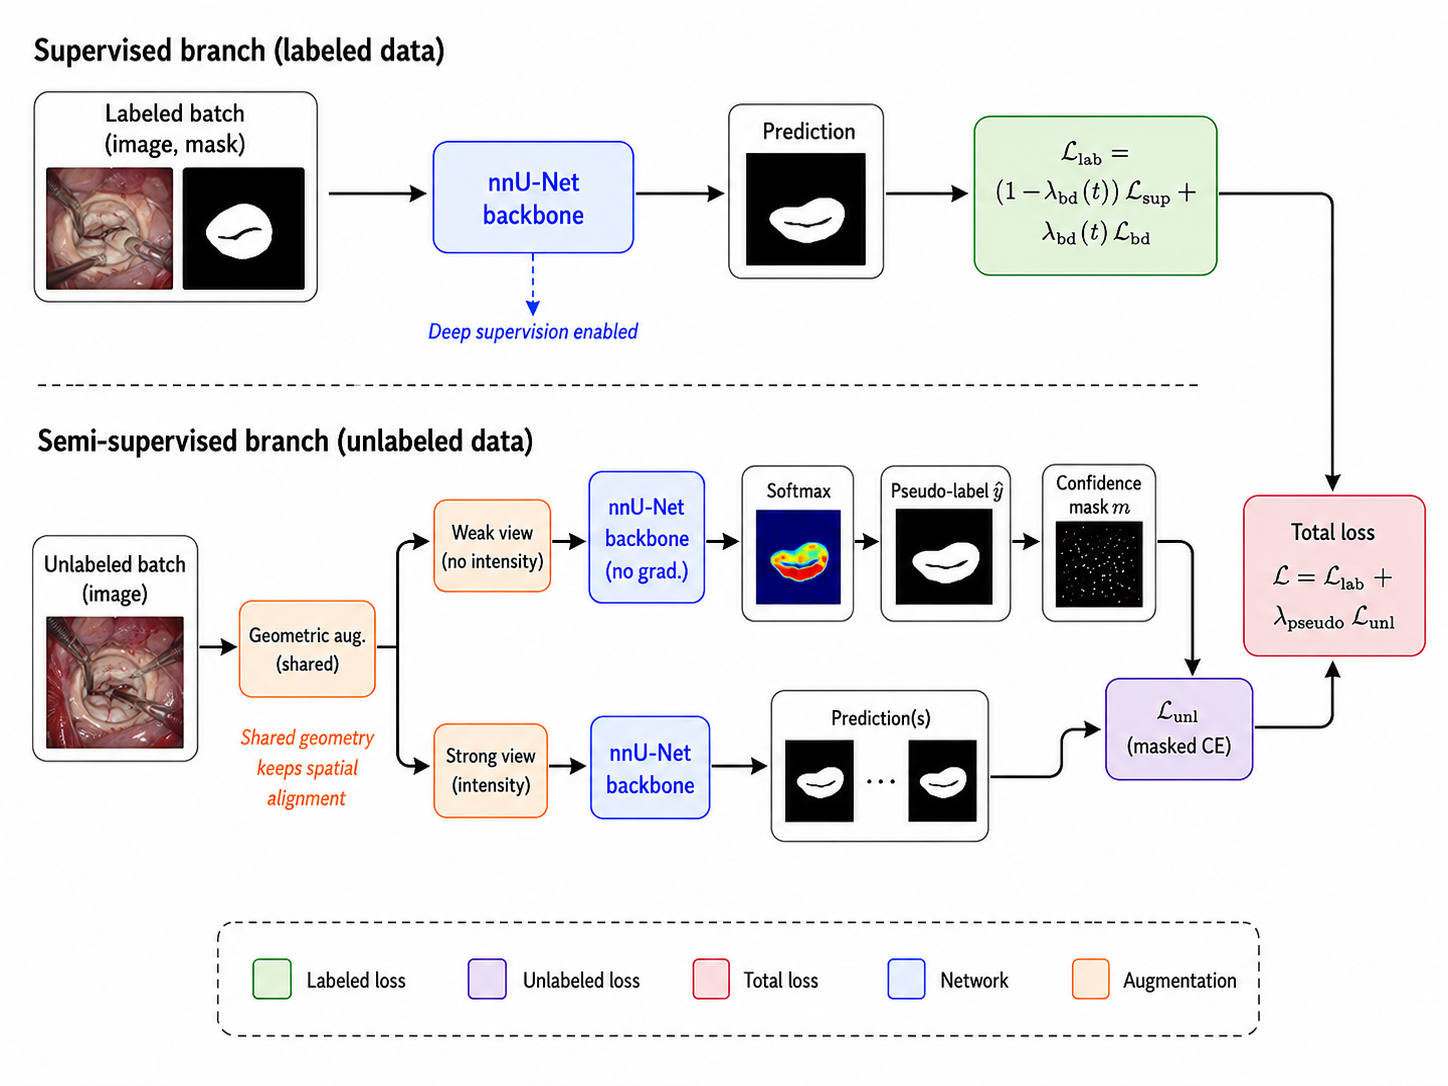
\includegraphics[width=\textwidth]{concept_figure.png}
\caption{Overview of the proposed framework for the surgical video frame~(Task~3) images. Labeled data use Dice,
cross-entropy, and boundary losses. For unlabeled data, the weak view
generates confidence-filtered pseudo-labels, while the
intensity-augmented strong view is trained to match them.}
\label{fig:method}
\end{figure}

\subsection{Backbone and Supervised Objective}

The framework is based on nnU-Net~\cite{ref_nnunet}, which
automatically selects the image spacing, patch size, batch size, and
network configuration for each task. A 3D full-resolution network is
used for cardiac CT (Task~1) and 3D~TEE (Task~2), while a 2D network
is used for surgical video (Task~3). Deep supervision is retained with
nnU-Net's default weighting for the supervised branch.

Let $(x_l,y_l)$ denote a labeled image and its reference mask, and let
$p_l=\operatorname{softmax}(f_\theta(x_l))$ denote the network
prediction. The supervised objective combines soft Dice loss and
cross-entropy:

\begin{equation}
\mathcal{L}_{\mathrm{sup}}
=
\mathcal{L}_{\mathrm{Dice}}(p_l,y_l)
+
\mathcal{L}_{\mathrm{CE}}(p_l,y_l).
\end{equation}

\subsubsection{Boundary refinement.}

Small errors along the thin annulus and leaflet boundaries may have
little effect on region-overlap losses. A multi-class boundary
loss~\cite{ref_boundary} is therefore added. Let
$\mathcal{C}_{\mathrm{fg}}$ denote the set of foreground classes,
$p_{l,c}(q)$ the predicted probability for class $c$ at location $q$,
and $\phi_{y_l,c}(q)$ the signed distance map of the corresponding
reference class. The boundary loss is averaged over the foreground
classes:

\begin{equation}
\mathcal{L}_{\mathrm{bd}}
=
\frac{1}
{|\mathcal{C}_{\mathrm{fg}}||\Omega|}
\sum_{c\in\mathcal{C}_{\mathrm{fg}}}
\sum_{q\in\Omega}
\phi_{y_l,c}(q)\,
p_{l,c}(q),
\end{equation}

where $\Omega$ denotes the image domain. Boundary loss alone does not
ensure a valid foreground prediction and is therefore combined with
the supervised region loss:

\begin{equation}
\mathcal{L}_{\mathrm{lab}}(t)
=
\bigl(1-\lambda_{\mathrm{bd}}(t)\bigr)
\mathcal{L}_{\mathrm{sup}}
+
\lambda_{\mathrm{bd}}(t)
\mathcal{L}_{\mathrm{bd}}.
\end{equation}

The boundary-loss weight increases linearly over the training schedule:

\begin{equation}
\lambda_{\mathrm{bd}}(t)
=
\lambda_{\mathrm{bd}}^{\max}
\min\left(1,\frac{t}{T}\right),
\end{equation}

where $t$ is the current epoch and $T=300$ is the total number of
training epochs. The signed distance maps are recalculated after
spatial augmentation to keep them aligned with the augmented reference
masks.

\subsection{Weak--Strong Consistency on Unlabeled Data}

The semi-supervised branch in Fig.~\ref{fig:method} follows a
FixMatch-style approach~\cite{ref_fixmatch}. Let $x_u$ denote an
unlabeled image. A shared geometric transformation $T_g$ produces the
weak view $x_u^w=T_g(x_u)$. The strong view is defined as
$x_u^s=T_I(T_g(x_u))$, where $T_I$ denotes intensity augmentation.
Using the same geometric transformation keeps the weak and strong views
spatially aligned.

The weak prediction
$p^w=\operatorname{softmax}(f_\theta(x_u^w))$ is calculated without
gradient tracking. At each location $q$, the pseudo-label and
confidence mask are defined as

\begin{equation}
\hat{y}(q)
=
\operatorname*{arg\,max}_{c}p_c^w(q),
\qquad
m(q)
=
\mathbf{1}
\left[
\max_c p_c^w(q)\geq\tau
\right],
\end{equation}

where $\tau$ is the confidence threshold. The strong prediction
$p^s=\operatorname{softmax}(f_\theta(x_u^s))$ is calculated with
gradient tracking. The unlabeled objective is the masked cross-entropy
between the strong-view prediction and the weak-view pseudo-label:

\begin{equation}
\mathcal{L}_{\mathrm{unl}}
=
\frac{
\sum_{q\in\Omega}
m(q)\,
\mathcal{L}_{\mathrm{CE}}
\left(p^s(q),\hat{y}(q)\right)
}{
\sum_{q\in\Omega}m(q)+\varepsilon
},
\end{equation}

where $\varepsilon$ prevents division by zero. Only predictions above
the confidence threshold contribute to the loss. Deep supervision is
disabled for the unlabeled branch because pseudo-labels are available
only at the final output resolution. The shared geometric
transformation preserves spatial alignment, while intensity
augmentation makes the strong view more difficult. Matching the
strong-view prediction to the weak-view pseudo-label encourages stable
predictions under intensity changes.

\subsection{Total Objective}

The labeled and unlabeled losses are combined as

\begin{equation}
\mathcal{L}(t)
=
\mathcal{L}_{\mathrm{lab}}(t)
+
\mathbf{1}[t\geq t_{\mathrm{warm}}]\,
\lambda_{\mathrm{pseudo}}\,
\mathcal{L}_{\mathrm{unl}},
\end{equation}

where $t_{\mathrm{warm}}$ is the warmup duration and
$\lambda_{\mathrm{pseudo}}$ controls the contribution of the unlabeled
loss. Before $t_{\mathrm{warm}}$, training uses labeled data only,
allowing the model to learn an initial segmentation before
pseudo-labeling begins.

The fully labeled 3D~TEE task uses only
$\mathcal{L}_{\mathrm{lab}}$, while cardiac CT and surgical video use
both loss terms. The task-specific values of
$\lambda_{\mathrm{pseudo}}$ and $\lambda_{\mathrm{bd}}^{\max}$ are
reported in Section~\ref{sec:experiments}.

\section{Dataset}
\label{sec:data}

The MVAA challenge dataset contains three independent tasks covering
cardiac CT, 3D~TEE, and intraoperative surgical video. All reference
annotations were created by clinical experts. Task~1 contains 1{,}067
3D cardiac CT scans, with the mitral annulus and anterior and posterior
leaflets annotated in 27 scans; the remaining 1{,}040 scans are
unlabeled, and 30 additional scans form the validation set. Task~2
contains 105 fully labeled 3D~TEE volumes with two leaflet classes and
20 validation volumes. Task~3 contains 1{,}559 surgical video frames,
of which 180 are labeled and 1{,}379 are unlabeled. Among the labeled
frames, 118 contain the mitral valve and are used for supervised
training. The remaining 62 labeled frames do not contain a visible
valve and are excluded from training. The video validation set contains
48 frames, all showing the valve. Semi-supervised learning is used for
Tasks~1 and~3, while Task~2 uses only supervised training.
Table~\ref{tab:data} summarizes the dataset sizes and the labeled
samples used for training.

\begin{table}[t]
\caption{Dataset size and number of labeled samples used for training.
Validation labels are held out by the challenge organizers.}
\label{tab:data}
\centering
\begin{tabular}{llllll}
\toprule
Task & Modality & Labeled & Used & Unlabeled & Validation \\
\midrule
Task~1 & Cardiac CT     & 27  & 27  & 1{,}040 & 30 \\
Task~2 & 3D TEE         & 105 & 105 & --      & 20 \\
Task~3 & Surgical video & 180 & 118 & 1{,}379 & 48 \\
\bottomrule
\end{tabular}
\end{table}

\section{Experiments}
\label{sec:experiments}

\subsection{Implementation Details}

The preprocessing, target spacing, patch size, and batch size selected
by nnU-Net are used for each task. The 3D full-resolution
configuration is applied to cardiac CT and 3D~TEE, while the 2D
configuration is used for surgical video. All models are trained from
scratch for 300 epochs with mixed precision using stochastic gradient
descent, Nesterov momentum of $0.99$, an initial learning rate of
$0.01$, weight decay of $3\times10^{-5}$, and nnU-Net's polynomial
learning-rate schedule. Deep supervision is enabled for the supervised
branch. Supervised video training uses only the 118 labeled frames that
contain the mitral valve. For unlabeled data, one shared spatial
transformation produces the weak view, while the strong view receives
the same spatial transformation together with intensity augmentation.
The confidence threshold is $\tau=0.95$, the unlabeled loss begins
after a 20-epoch warmup, and the boundary-loss weight increases
linearly over the 300-epoch training schedule. No separate internal
validation set or model-selection experiment is used. The reported
settings are used for the final training runs. Table~\ref{tab:cfg}
reports the task-specific loss weights.

\begin{table}[t]
\caption{Task-specific loss weights. Shared settings are the default
nnU-Net plans, $\tau=0.95$, a 20-epoch warmup, 300 training epochs,
an initial learning rate of $0.01$, weight decay of
$3\times10^{-5}$, and one weak and one strong unlabeled view.}
\label{tab:cfg}
\centering
\begin{tabular}{lllll}
\toprule
Task & Modality & Config & $\lambda_{\mathrm{pseudo}}$ &
$\lambda_{\mathrm{bd}}^{\max}$ \\
\midrule
Task~1 & Cardiac CT      & 3d\_fullres & 0.25 & 0.10 \\
Task~2 & 3D TEE          & 3d\_fullres & --   & 0.01 \\
Task~3 & Surgical video  & 2d          & 0.10 & 0.01 \\
\bottomrule
\end{tabular}
\end{table}

\section{Results}
\label{sec:results}

Table~\ref{tab:results} summarizes performance on the three validation
sets. Segmentation overlap is measured using the Dice similarity
coefficient (DSC)~\cite{ref_dice,ref_taha_metrics}, while boundary
accuracy is measured using the 95th-percentile Hausdorff distance
(HD95) and average surface distance
(ASD)~\cite{ref_hausdorff,ref_taha_metrics}. Higher DSC and lower HD95
and ASD indicate better segmentation. HD95 and ASD are reported in
millimetres using the spatial information provided for each image. For
each validation case, every metric is calculated separately for each
foreground class and then averaged across the foreground classes. The
reported task-level values are the means across all validation cases.

\begin{table}[t]
\caption{Validation performance of the proposed framework. HD95 and
ASD are reported in millimetres.}
\label{tab:results}
\centering
\begin{tabular}{lcccc}
\toprule
Task & DSC $\uparrow$ & HD95 (mm) $\downarrow$ &
ASD (mm) $\downarrow$ & Cases \\
\midrule
Task~1: Cardiac CT      & 0.834 & 7.660   & 0.339  & 30 \\
Task~2: 3D TEE          & 0.789 & 23.716  & 2.060  & 20 \\
Task~3: Surgical video  & 0.649 & 172.345 & 29.528 & 48 \\
\bottomrule
\end{tabular}
\end{table}

Cardiac CT produced a DSC of 0.834, an HD95 of 7.660~mm, and an ASD
of 0.339~mm. The high overlap and low surface-distance values indicate
close agreement between the predicted and reference CT segmentations.
For 3D~TEE, the framework achieved a DSC of 0.789, an HD95 of
23.716~mm, and an ASD of 2.060~mm. The difference between ASD and
HD95 indicates that the upper end of the boundary-error distribution
was larger than the average boundary error.

Surgical video produced a DSC of 0.649, an HD95 of 172.345~mm, and an
ASD of 29.528~mm. The lower overlap and larger surface-distance values
indicate errors in both valve localization and boundary delineation.
Direct numerical comparison across the three tasks should be made with
care because the imaging modalities, target structures, numbers of
classes, and spatial scales differ. All expected validation cases were
processed, with no missing predictions.

Only the complete framework was evaluated. Without labeled-only
baselines or ablation experiments, the results cannot isolate the
effects of weak--strong consistency learning or boundary refinement.

\section{Conclusion}
\label{sec:conclusion}

A semi-supervised framework for mitral valve segmentation was developed
using nnU-Net, weak--strong consistency learning, and multi-class
boundary refinement. Separate models were trained for cardiac CT,
3D~TEE, and surgical video, with unlabeled data used only for the CT
and video tasks. The task-specific evaluations showed high overlap and
low surface errors for cardiac CT, moderate performance for 3D~TEE,
and larger localization and boundary errors for surgical video.
However, direct comparison across the tasks is limited by differences
in imaging modality, target definition, class structure, and spatial
scale.

The framework provides a simple way to combine labeled and unlabeled
data without a separate teacher network or a manually designed
modality-specific architecture. The current study does not include a
separate internal validation set, a labeled-only baseline, or an
ablation analysis. Future work should include internal cross-validation,
supervised baselines, and component-wise ablation experiments to assess
hyperparameter robustness and measure the separate contributions of
consistency learning and boundary refinement.

% Acknowledgements and competing-interests statements are omitted in the
% anonymized submission and will be added in the camera-ready version.
%
% ---- Bibliography ----
%
\bibliographystyle{splncs04}
\bibliography{reference}
%
\end{document}
